% Carattere dimensione 12
\documentclass[12pt]{report}

% Margini (2.5cm su tutti i lati)
\usepackage[top=2.5cm, bottom=2.5cm, left=2.5cm, right=2.5cm, head=21.75pt, centering]{geometry}

% Interlinea
\linespread{1.5}
\usepackage[italian]{babel} % applicazione regole di scrittura per la lingua italiana
\usepackage[utf8]{inputenc} % codifica UTF-8
\usepackage{scrlayer-scrpage} % stili pagina per il frontespizio
\ifoot[]{}
\cfoot[]{}
\ofoot[\pagemark]{\pagemark}
\pagestyle{scrplain} 
\usepackage[hidelinks]{hyperref} % pacchetto per l'utilizzo dei link
\usepackage[T1]{fontenc}
\usepackage{inconsolata}
\usepackage{newtxtext,newtxmath} % font Times New Roman (simile)
\usepackage{csquotes} % per le citazioni "in blocco"
\usepackage{booktabs}    
\usepackage{adjustbox}  
\usepackage{filehook}
\usepackage{makecell}    
\usepackage[bottom]{footmisc}
\usepackage{pifont}  
\usepackage[utf8]{inputenc}
\usepackage{subcaption} % per le sottofigure
\usepackage[backend=bibtex]{biblatex} % bibliografia con pacchetto biblatex
\usepackage{verbatim} % per usare \begin{comment} \end{comment}
\usepackage{multirow}
\appto{\bibsetup}{\raggedright}
\addbibresource{bibliography.bib} % Collega il file della bibliografia

\usepackage{titlesec} % per la formattazione dei titoli delle sezioni, capitoli etc.
\usepackage{float} % per il posizionamento delle immagini

\usepackage{listings} % per il codice di programmazione
\usepackage{minted}
\usepackage{color}
\usepackage{xcolor}
\usepackage{xurl}
% \usepackage{tikz}
% \usetikzlibrary{calc}
\usepackage{booktabs} % for \toprule, \midrule, \bottomrule in tables
\usepackage{algorithm}
\usepackage{algpseudocode}
\usepackage{graphicx}

% Definizione dei colori per il codice
\definecolor{lightgray}{rgb}{.9,.9,.9}
\definecolor{darkgray}{rgb}{.4,.4,.4}
\definecolor{purple}{rgb}{0.65, 0.12, 0.82}
\definecolor{mygreen}{rgb}{0,0.6,0}
\definecolor{mygray}{rgb}{0.5,0.5,0.5}
\definecolor{mymauve}{rgb}{0.58,0,0.82}
\definecolor{backcolour}{rgb}{0.95,0.95,0.92}

% Stili per i linguaggi di programmazione
\lstdefinelanguage{JavaScript}{
  keywords={typeof, new, true, false, catch, function, return, null, catch, switch, var, let, const, if, in, while, do, else, case, break},
  keywordstyle=\color{blue}\bfseries,
  ndkeywords={class, export, boolean, throw, implements, import, this},
  ndkeywordstyle=\color{darkgray}\bfseries,
  identifierstyle=\color{black},
  sensitive=false,
  comment=[l]{//},
  morecomment=[s]{/*}{*/},
  morestring=[b]',
  morestring=[b]",
  commentstyle=\color{mygreen}\ttfamily,
  stringstyle=\color{mymauve}\ttfamily,
  backgroundcolor=\color{backcolour},
  basicstyle=\footnotesize\ttfamily,
  showstringspaces=false,
  extendedchars=true,
  showspaces=false,
  numbers=left,
  numberstyle=\footnotesize,
  numbersep=9pt,
  tabsize=2,
  breaklines=true,
  showtabs=false,
  captionpos=b
}

\lstdefinelanguage{MyPython}{
  language=Python,
  morekeywords={with, as},
  keywordstyle=\bfseries\color{blue},
  commentstyle=\color{mygreen},
  stringstyle=\color{mymauve},
  backgroundcolor=\color{backcolour},
  basicstyle=\footnotesize\ttfamily,
  showstringspaces=false,
  numbers=left,
  numberstyle=\footnotesize,
  numbersep=9pt,
  tabsize=2,
  breaklines=true,
  showtabs=false,
  captionpos=t
}

\lstdefinestyle{bash}{
    basicstyle=\ttfamily\small,
    rulesepcolor=\color{black},
    language=bash,
    breaklines=true,
    backgroundcolor=\color{backcolour},
    literate={"}{{\texttt{"}}}{1},
    numbers=left,
    numberstyle=\footnotesize,
    numbersep=9pt,
    columns=fixed,
    keepspaces=true,
}

\lstdefinestyle{Prompt}{
  breaklines=true,
  basicstyle=\ttfamily,
}

\lstdefinestyle{Myyaml}{
  basicstyle=\ttfamily\small,
  breaklines=true,
  numbers=left,
  numberstyle=\footnotesize,
  numbersep=9pt,
  showstringspaces=false,
  tabsize=2,
  backgroundcolor=\color{backcolour},
  columns=fixed,
  keepspaces=true,
}

% Formato delle intestazioni
\titleformat{\chapter}[block]
  {\normalfont\LARGE\bfseries}{\thechapter.}{0.5em}{\LARGE}
\titlespacing*{\chapter}{0pt}{-20pt}{25pt}


\usepackage{enumitem}

\begin{document}
    \begin{titlepage}
    
        \begin{center}
            
\includegraphics[width=8cm]{images/unimore/Sigillo2015.png}
            \vspace{1cm}
    
            {\LARGE{ UNIVERSITÀ DEGLI STUDI DI MODENA \\E REGGIO EMILIA \\}}
            {\large{ Dipartimento di Scienze Fisiche, Informatiche e Matematiche \\}}
            {\large{ Corso di Laurea Magistrale in Informatica (LM-18) \\}}
            \vspace{3cm}
            {\Large { \textbf{Floorplan3D:  implementazione di una pipeline per la generazione di mesh 3D a partire da modelli CAD 2D di planimetrie architettoniche} }}\\
            \vspace{3cm}
        \end{center}
        
        \begin{minipage}[t]{0.47\textwidth}
        	{\large{\bf Relatore:}\\} 
            {\large Prof. Nicola Capodieci\\}
            {\large{\bf Correlatore:}\\} 
            {\large Prof. Fabio Pellacini\\}
        \end{minipage}\hfill\begin{minipage}[t]{0.47\textwidth}\raggedleft
        	{\large{\bf Candidato:}\\}
            {\large Simone Vaiasinni}\\
            {\large Matricola 201711}
        \end{minipage}
        
        \vfill
        \hrulefill\\
        \centering{\large{\bf ANNO ACCADEMICO 2025/2026 }}
    \pagenumbering{roman}
    \end{titlepage}
    \newpage
    \thispagestyle{empty}
    \null
    \newpage
    \pagestyle{empty}
    \makeatletter
\newcommand{\beginitalianAbstract}{%
  \thispagestyle{plain}%
  \begin{center}
    \setlength{\parskip}{0pt}
    {\huge\textit{Abstract}\par}
    \bigskip
    {\normalsize\bf \ttitle \par}
    \bigskip
  \end{center}
}
\makeatother

\newcommand{\ttitle}{Floorplan3D:  implementazione di una pipeline per la generazione di mesh 3D a partire da modelli CAD 2D di planimetrie architettoniche}

\beginitalianAbstract
\addcontentsline{toc}{chapter}{Abstract}

L'abstract è il riassunto della tesi. Deve dare in poche righe (in genere 150-300 parole, una mezza pagina), una visione completa e autosufficiente del lavoro: problema, approccio, risultati, senza bisogno di leggere il resto.

1. Contesto e problema (2-3 righe)
Qual è il problema generale? Perché è rilevante? Nel tuo caso: la difficoltà di ottenere modelli 3D di ambienti architettonici a partire da planimetrie 2D CAD, utili per rendering, visualizzazione, ecc.

2. La sfida specifica (1-2 righe)
Cosa rende il problema difficile? Nel tuo caso: l'assenza di uno standard unico tra i modelli CAD, che rende difficile generalizzare un algoritmo.

3. Cosa hai fatto (il cuore dell'abstract, 4-6 righe)
Qui descrivi Floorplan3D: un sistema/pipeline che, a partire da un file DXF con muri, porte e finestre, produce una mesh 3D esportata in GLTF. Vale la pena accennare, senza entrare troppo nei dettagli implementativi, alle fasi principali della pipeline (parsing, ricostruzione geometrica dei varchi, estrazione del grafo planare e delle facce, triangolazione ed estrusione), perché è proprio questo il contributo tecnico del lavoro.

4. Risultati/validazione (1-2 righe)
Cosa hai ottenuto? Hai testato su più planimetrie reali? Hai fatto un confronto qualitativo, dei rendering finali in Blender, delle metriche sui tempi di elaborazione, sulla qualità della mesh? Anche un risultato qualitativo ("il sistema produce mesh corrette e prive di artefatti su planimetrie reali di complessità variabile") va benissimo se non hai metriche quantitative.


 
    \clearpage
    
    \pagestyle{empty}
    \clearpage
    
    \tableofcontents      % Generates the Table of Contents
    \renewcommand{\listfigurename}{Elenco delle Figure}
    \listoffigures        % Generates the List of Figures
    \renewcommand{\lstlistingname}{Code}
    \renewcommand{\lstlistlistingname}{Elenco dei Codici}

    \lstlistoflistings    % Generates the List of Code Listings
    
    \clearpage
    \pagestyle{scrplain} % Restores the normal page style (with page number)
    \setcounter{page}{1} % Restart page numbering from 1
    \pagenumbering{arabic}
    % Add chapters here
    \chapter{Introduzione}
\label{ch:introduzione}

L'obiettivo del presente lavoro di tesi è quello di sviluppare un sistema in grado di generare automaticamente una mesh 3D partendo da un modello CAD 2D di una planimetria di una singola stanza o di un appartamento.

Per ogni modello CAD 2D che verrà letto in input dal sistema il risultato sarà una mesh 3D con vertici, indici, normali e coordinate di texture che possono essere immediatamente utilizzate per il rendering.

Il dominio del problema comprende i piani architettonici CAD 2D in formato DXF (Drawing Exchange Format). Per poter iniziare a lavorare sulla progettazione della pipeline di elaborazione è stato prima necessario raccogliere un dataset composto da modelli CAD 2D rappresentativi del dominio di applicazione, più di dieci modelli CAD sono stati raccolti da diversi siti web come \texttt{draftsperson.net}, \texttt{pincad.com} e \texttt{archweb.com}.
Questi modelli CAD erano inizialmente disponibili nel formato DWG e sono quindi stati convertiti in formato DXF e poi controllati con un software di editing come LibreCAD.

Mentre DWG e DXF sono standard de facto nel campo del CAD sono diversi tra loro per quanto riguarda l'approccio alla codifica: DWG è un formato binario proprietario, più efficiente nello spazio ma meno leggibile in quanto può essere letto da poche applicazioni, mentre DXF è un formato basato sul testo (in ASCII) sviluppato in modo tale da non presentare problemi di interoperabilità con i software di terzi. \cite{adobe_dwg_dxf} Tra i modelli disponibili ne sono stati selezionati alcuni come studi di caso.

\section{I problemi dei modelli CAD: eterogeneità e mancanza di standard}
\label{sec:problemi_modelli_CAD}

Il formato DXF non fornisce direttamente poligoni, bensì un insieme di entità geometriche disconnesse tra loro, quali \texttt{POLYLINE}, \texttt{LINE}, \texttt{ARC}, \texttt{BLOCK} ecc., organizzate in layer identificati da un nome. È qui che emerge la prima criticità: non esiste alcuno standard che imponga una convenzione univoca sui nomi dei layer. Uno stesso layer contenente i muri può essere chiamato, a seconda del modello, \texttt{WALLS}, \texttt{A-WALL}, \texttt{WALL EXTERNAL}, \texttt{WALL INTERNAL}, e così via.

Un secondo problema riguarda la rappresentazione geometrica degli elementi. Non esiste uno standard neppure per la rappresentazione consistente dei muri: alcuni modelli li descrivono tramite polilinee, altri tramite semplici segmenti. Isolando le sole primitive relative ai muri, inoltre, si osservano ulteriori problemi ricorrenti: segmenti che si intersecano impropriamente tra loro, e contorni di muri che risultano aperti anziché chiusi.

Anche le finestre presentano una notevole variabilità rappresentativa: alcuni modelli le descrivono come blocchi complessi composti da migliaia di segmenti, altri come semplici segmenti che collegano due muri, altri ancora come rettangoli definiti da quattro segmenti. Le porte, al contrario, tendono a essere rappresentate in modo più uniforme tra i vari modelli, tipicamente tramite archi; nel caso peggiore, tuttavia, anche una porta, in particolare quella d'ingresso, può essere rappresentata tramite polilinee o segmenti anziché tramite un arco.

Questa eterogeneità è la ragione principale per cui non è possibile progettare un algoritmo generale in grado di elaborare correttamente qualsiasi modello CAD. È necessaria, a monte dell'elaborazione automatica, una fase di preprocessing volta a rendere il modello quanto più consistente possibile (Capitolo \ref{ch:geometry_processing}).

\section{Assunzioni progettuali}
\label{sec:assunzioni_progettuali}

Per affrontare queste criticità vengono fatte delle assunzioni ragionevoli, che consentono di semplificare il problema:
\begin{enumerate}
	\item i layer relativi a pareti, porte e finestre devono avere nomi riconoscibili (ad esempio \texttt{A-WALL}, \texttt{A-DOOR}, \texttt{A-WINDOW}). L'utente è tenuto a rinominarli manualmente;
	\item i muri devono essere già rappresentati come facce chiuse (poligoni), dotate di proprio spessore; eventuali \emph{crack} o discontinuità nei contorni devono essere riparate manualmente prima dell'esecuzione mediante software di editing CAD (come LibreCAD);
	\item le porte e finestre sono considerati buchi, o discontinuità,  nelle pareti e verranno trattati come tali durante la fase di estrusione, con altezze differenziate
\end{enumerate}

    \chapter{Progettazione e implementazione della pipeline geometrica}
\label{ch:geometry_processing}

\section{Preprocessing}
\label{sec:preprocessing}

Come discusso nel Capitolo~\ref{ch:introduzione}, la fase di preprocessing ha l'obiettivo di rendere il modello CAD quanto più consistente possibile prima dell'elaborazione. Si interviene correggendo i layer, blocchi, geometrie e ridondanze.

Come caso di studio prendiamo il modello DXF selezionato e lo apriamo con LibreCAD per analizzarlo.

\begin{figure}[htbp]
	\centering
	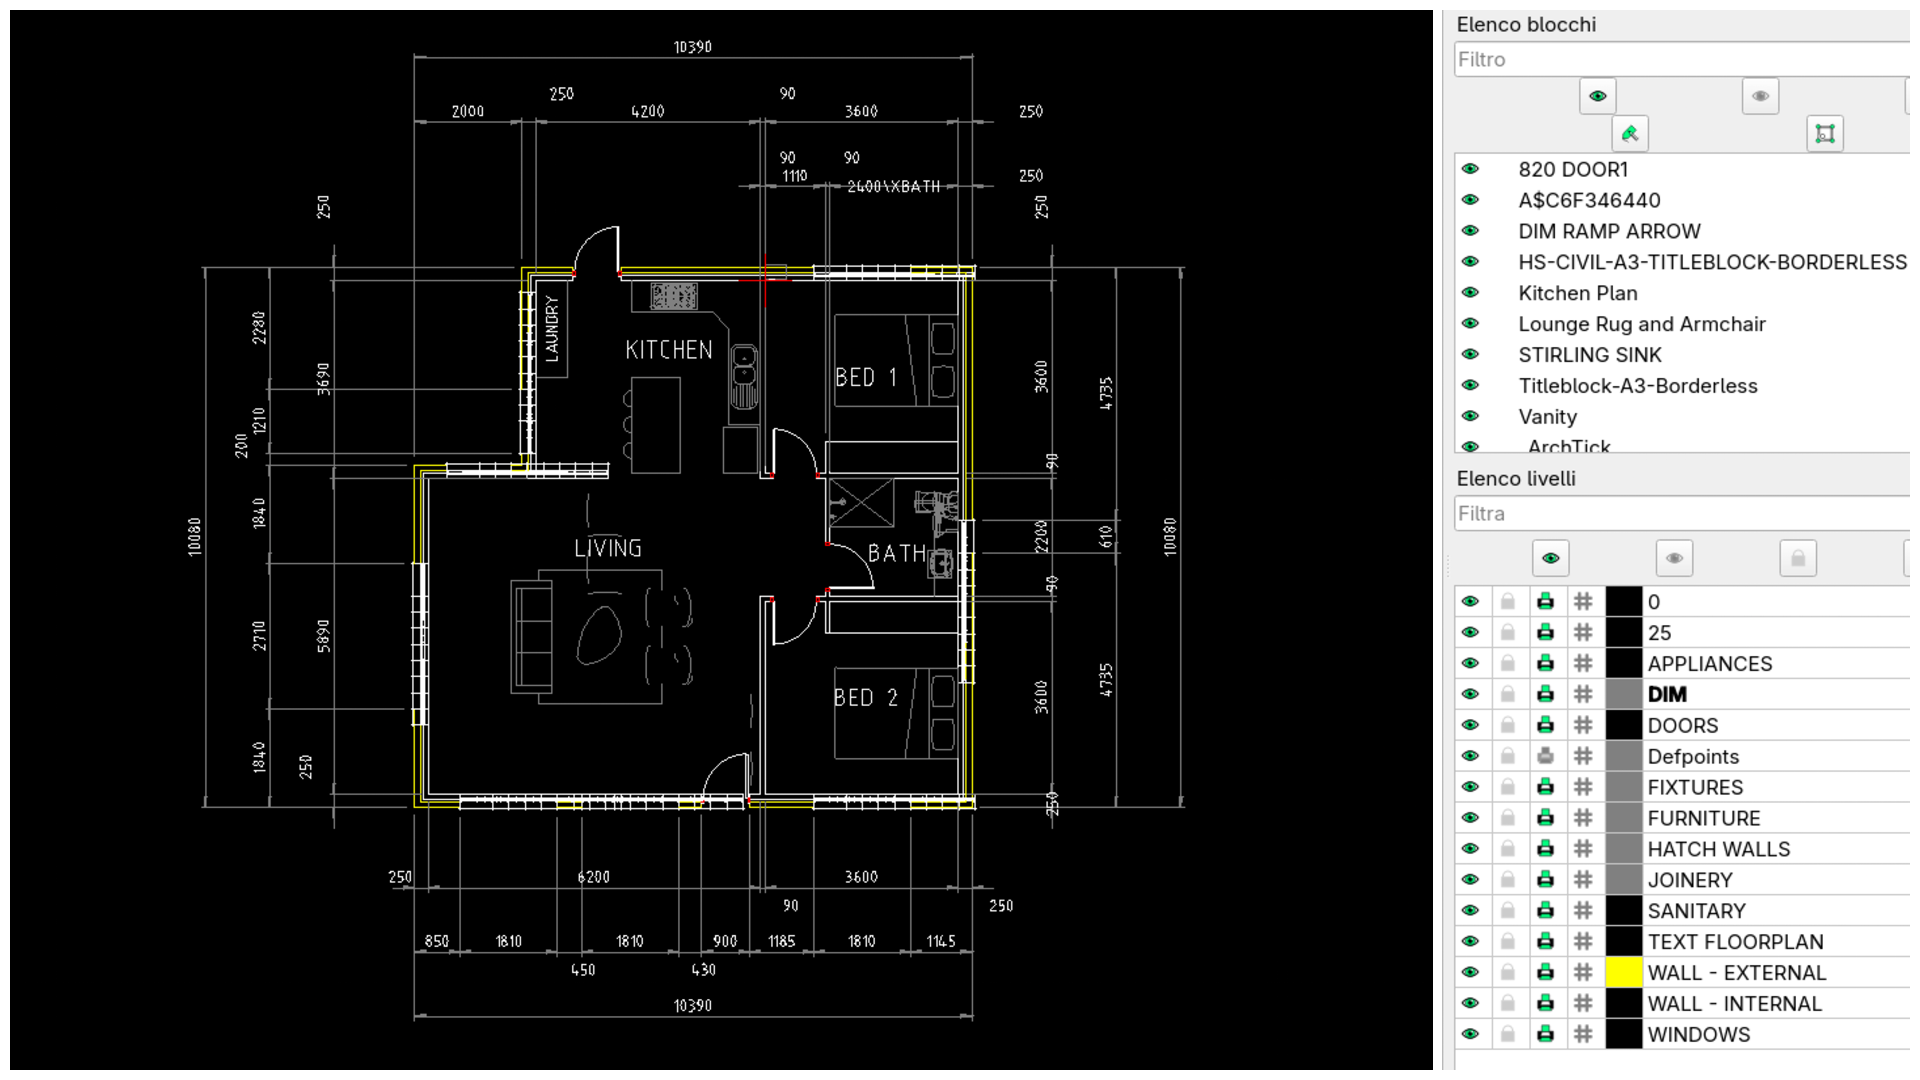
\includegraphics[width=1\textwidth]{images/02_geometry_processing/screen001.png}
	\caption{Modello CAD di caso di studio aperto in LibreCAD.}
	\label{fig:screen001}
\end{figure}

Isoliamo inizialmente solo i layer relativi ai muri e osserviamo che sono presenti due layer distinti: \texttt{WALL EXTERNAL} (evidenziato in giallo) e \texttt{WALL INTERNAL}. I segmenti del layer \texttt{WALL EXTERNAL} risultano ridondanti e possono essere rimossi senza alcun impatto sulla geometria finale. Osserviamo inoltre che le primitive dei muri non sono polilinee chiuse, bensì segmenti che formano contorni aperti: la geometria risulta quindi incompleta e necessita di correzione. Sono infine presenti due ulteriori segmenti isolati, che costituiscono rumore e possono anch'essi essere rimossi.

\begin{figure}[htbp]
	\centering
	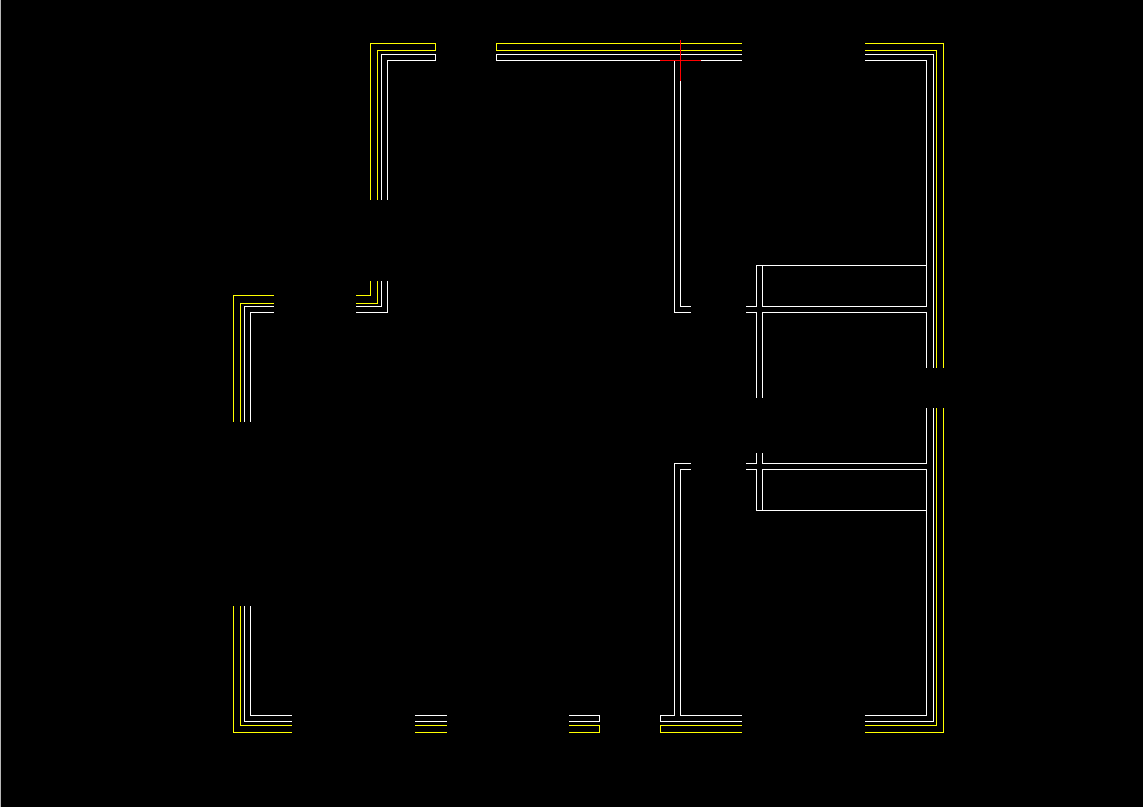
\includegraphics[width=0.7\textwidth]{images/02_geometry_processing/screen002.png}
	\caption{Layer dei muri prima della correzione: si notano il layer ridondante \texttt{WALL EXTERNAL}, i contorni aperti e i segmenti isolati.}
	\label{fig:screen002}
\end{figure}

Dopo aver corretto questi problemi, otteniamo la rappresentazione dei muri mostrata in figura:

\begin{figure}[htbp]
	\centering
	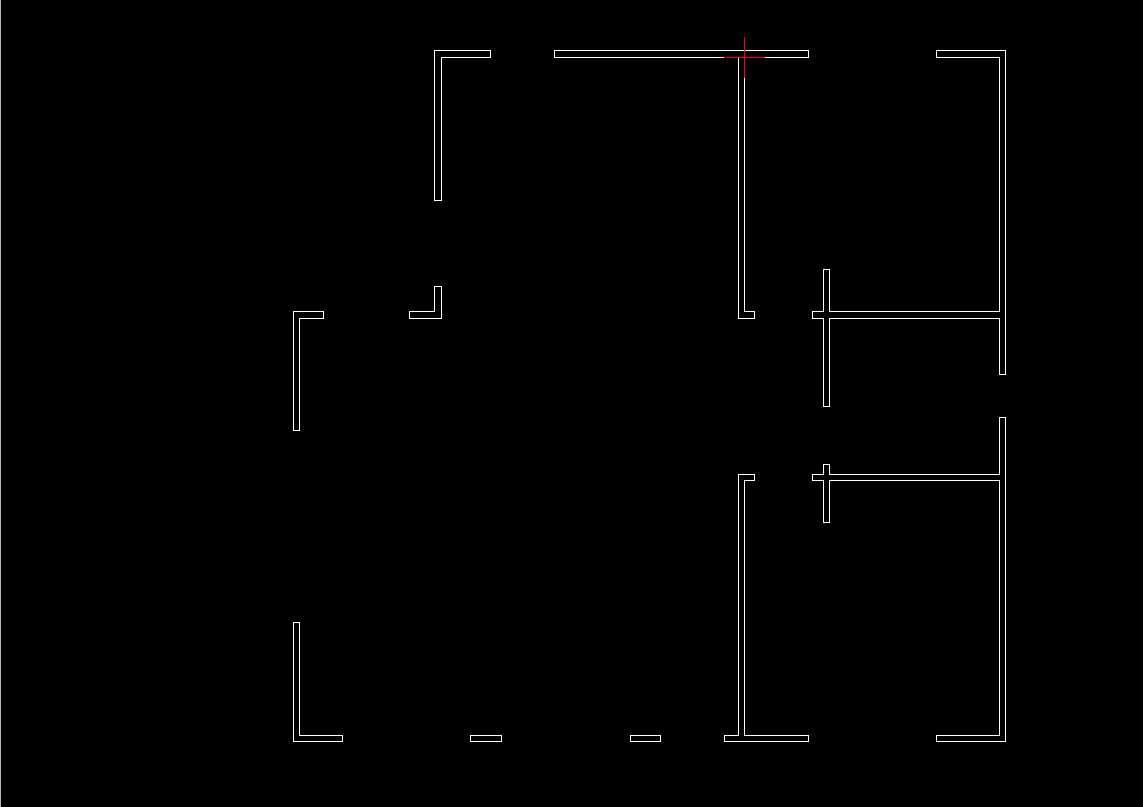
\includegraphics[width=0.7\textwidth]{images/02_geometry_processing/screen003.png}
	\caption{Layer dei muri dopo la correzione.}
	\label{fig:screen003}
\end{figure}

Nonostante i muri siano ancora separati tra loro, a causa della presenza di porte e finestre, quello che otteniamo è un insieme di poligoni chiusi. Analizziamo a questo punto le finestre: osserviamo come non siano rappresentate in una forma adeguata. Ogni finestra è descritta come un blocco (\texttt{BLOCK}) contenente centinaia di segmenti; inoltre, due finestre risultano sovrapposte tra loro, e due di queste fuoriescono addirittura dalle mura.

\begin{figure}[htbp]
	\centering
	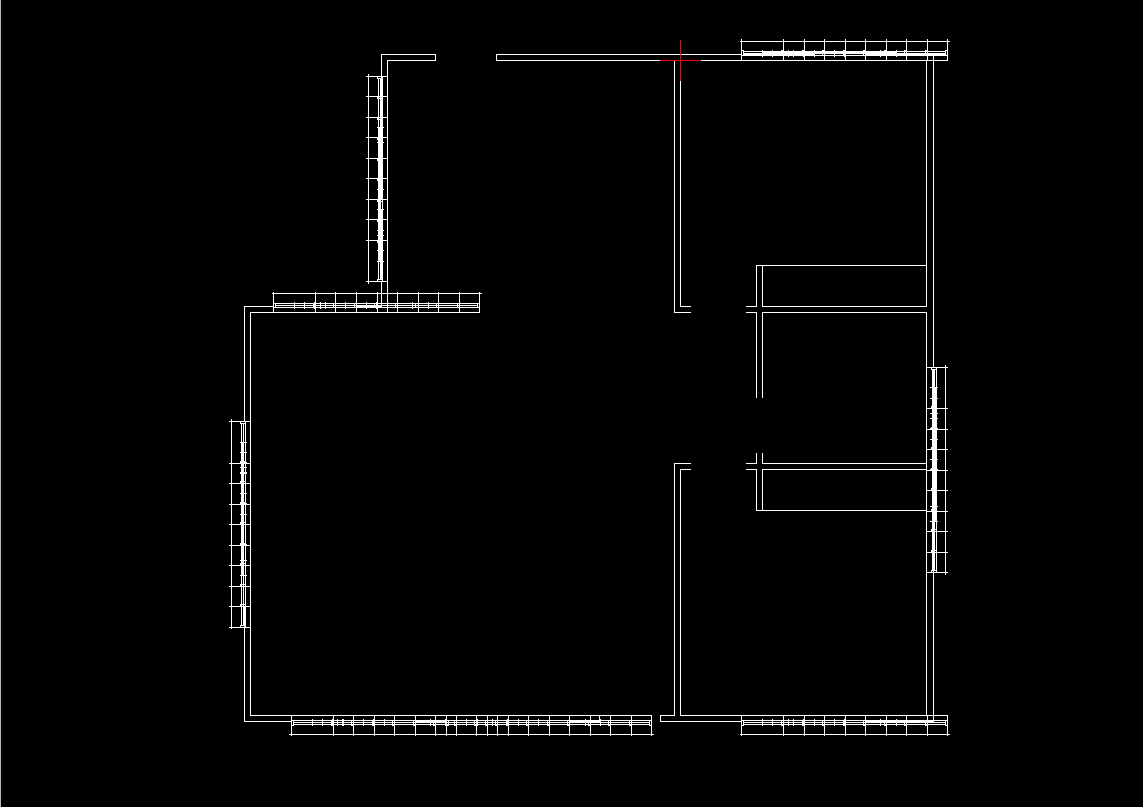
\includegraphics[width=0.7\textwidth]{images/02_geometry_processing/screen004.png}
	\caption{Rappresentazione originale delle finestre: si notano il blocco composto da centinaia di segmenti, la sovrapposizione tra due finestre e una finestra che invade lo spazio interno.}
	\label{fig:screen004}
\end{figure}

Dopodiché, i layer sono stati rinominati in modo coerente: \texttt{A-WALL} per i muri, \texttt{A-DOOR} per le porte e \texttt{A-WINDOW} per le finestre. Tutti gli altri layer, non essendo rilevanti per la ricostruzione della geometria, sono stati esclusi. Anche i blocchi sono stati rinominati: un blocco per la porta (\texttt{BLOCK-DOOR-1}) e quattro blocchi per le finestre (\texttt{BLOCK-WINDOW-1}, \ldots, \texttt{BLOCK-WINDOW-4}).

\begin{figure}[htbp]
	\centering
	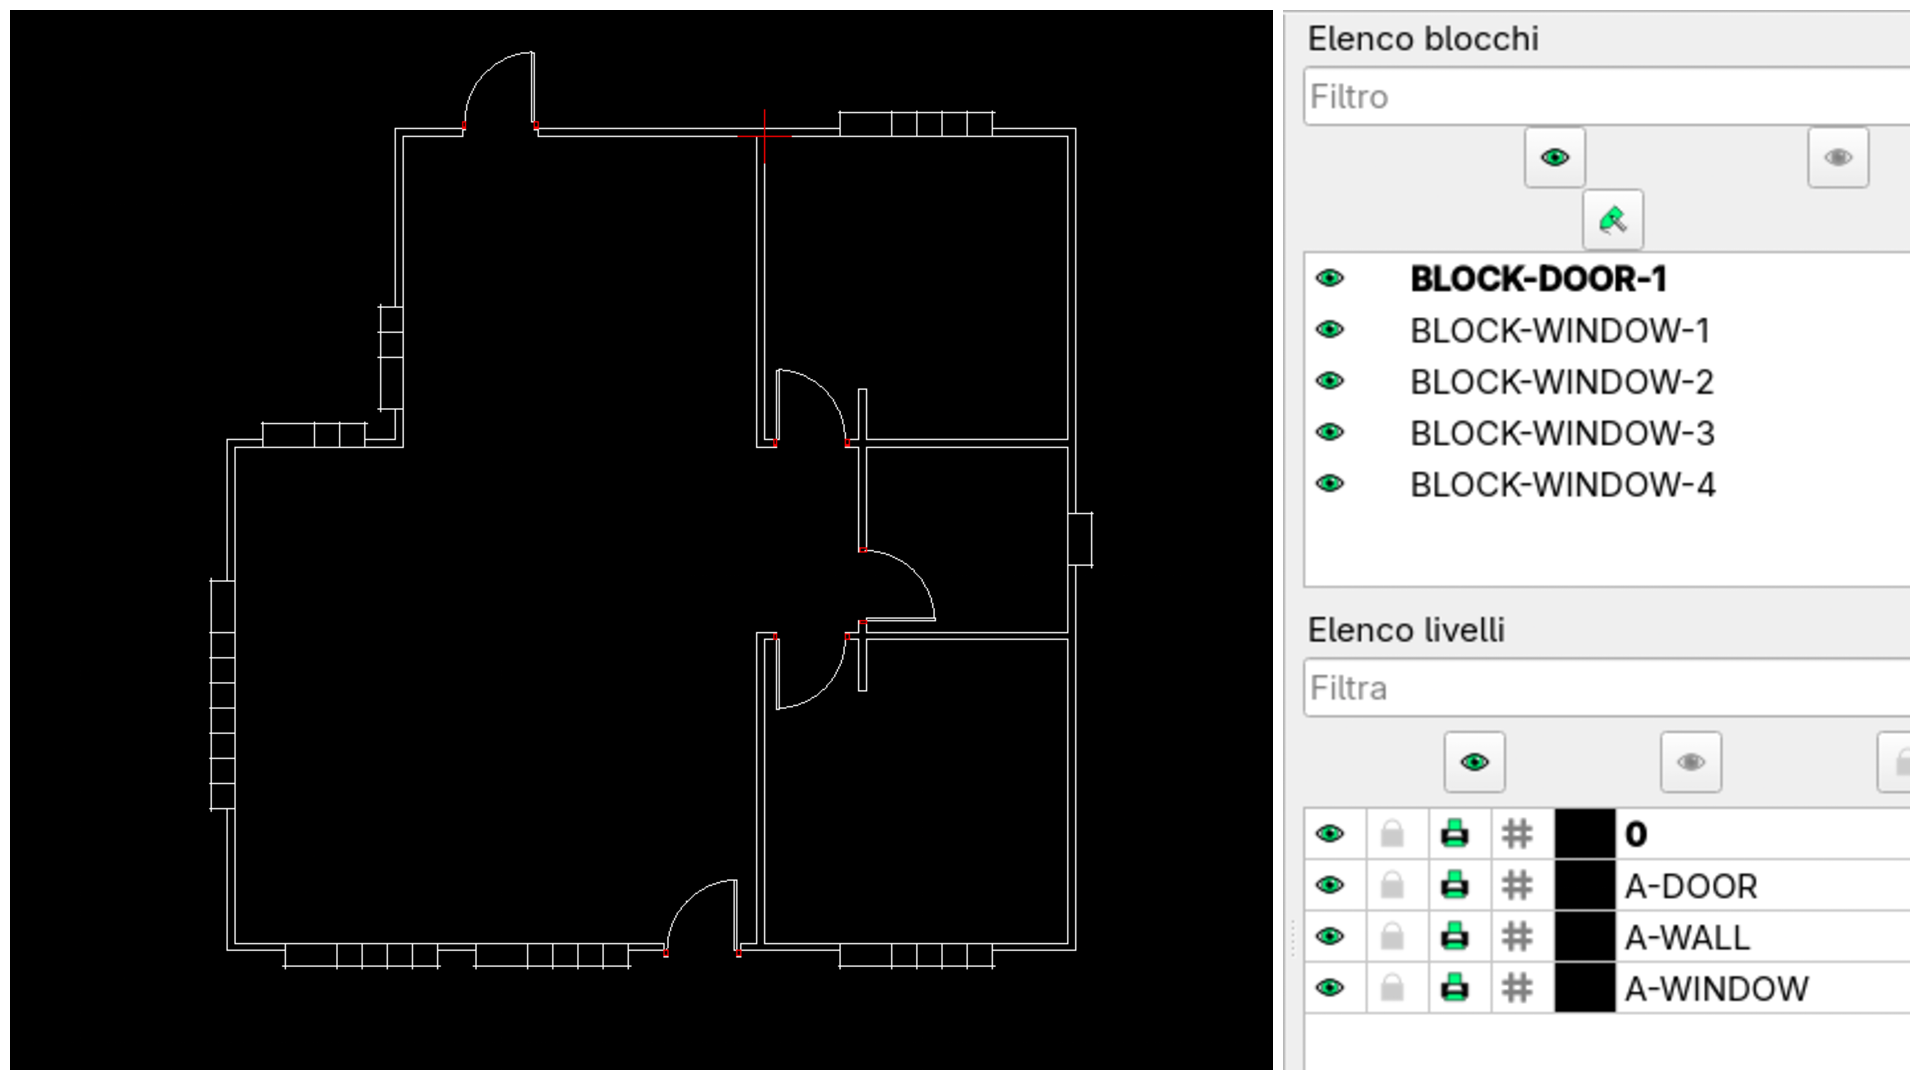
\includegraphics[width=0.7\textwidth]{images/02_geometry_processing/screen005.png}
	\caption{Rappresentazione delle finestre dopo la correzione.}
	\label{fig:screen005}
\end{figure}

\section{Parsing}
\label{sec:parsing}


Il formato DXF organizza il disegno in primitive geometriche: LINE, POLYLINE, ARC, CIRCLE ecc. Queste entità sono raggruppate in layer che consentono di separare logicamente i diversi elementi del disegno (ad esempio muri, porte, finestre, arredi, testo). Oltre ai layer, il formato DXF supporta i blocchi (BLOCK), che non sono altro che componenti riutilizzabili. Sono comunemente utilizzati per rappresentare porte e finestre. Un blocco viene definito una volta all'interno del file e può essere istanziato più volte tramite entità INSERT, ciascuna con una propria posizione, scala e rotazione. Questa funzionalità è particolarmente utile per rappresentare elementi ripetuti, come porte, finestre o arredi, che compaiono più volte nella stessa planimetria.

L'obiettivo della fase di parsing è estrarre da queste primitive le informazioni geometriche necessarie alla costruzione della mesh, e collassare tutte le primitive sotto forma di segmenti per avere una rappresentazione uniforme.

Si consideri il modello CAD corretto durante il preprocessing, che presenta layer standardizzati (\texttt{A-WALL}, \texttt{A-DOOR}, \texttt{A-WINDOW}) e blocchi rinominati (\texttt{BLOCK-DOOR-1}, \texttt{BLOCK-WINDOW-1}, \ldots, \texttt{BLOCK-WINDOW-4}).

Il parsing viene realizzato in C++ mediante la libreria open source \href{https://github.com/Codelibs/libdxfrw}{libdxfrw}, che fornisce un'interfaccia per la lettura dei file DXF. La classe del parser implementa le callback necessarie per gestire i diversi tipi di entità:
\begin{minted}[frame=single]{cpp}
enum class SegmentLayer : i32 { None=0, Wall, Window, Door };
struct Segment{ glm::dvec2 start, end; SegmentLayer layer; };
	
class DRWParser : public DRW_Interface
{
public:
  virtual void addLine(const DRW_Line& data) override;
  virtual void addLWPolyline(const DRW_LWPolyline& data) override;
  virtual void addArc(const DRW_Arc& data) override;
  virtual void addInsert(const DRW_Insert& data) override;
  virtual void addBlock(const DRW_Block& data) override;
  virtual void endBlock() override;
	
  virtual void addHatch([[maybe_unused]]const DRW_Hatch* data) override {}
  virtual void addCircle([[maybe_unused]]const DRW_Circle& data) override {}
  ...
  SegmentLayer classify_layer(std::string_view name);	
  std::vector<Segment> walls, doors, windows;
};
\end{minted}

Tra le callback messe a disposizione, quelle che ci interessano maggiormente sono:
\begin{itemize}
	\item \texttt{addLine()}: viene invocata per ogni segmento (\texttt{LINE}) presente nel disegno. I due punti estremi vengono memorizzati direttamente come segmento;
		
	\item \texttt{addLWPolyline()}: per le polilinee (\texttt{LWPolyline}), si iterano i vertici della polilinea per generare una sequenza di segmenti consecutivi;
	
	\item \texttt{addArc()}: per gli archi (\texttt{ARC}), si estraggono il raggio, il punto base, l'angolo iniziale e l'angolo finale. A partire da questi dati, si calcolano i due punti estremi dell'arco, che corrispondono agli spigoli delle pareti; il segmento che li collega costituisce la rappresentazione della porta;
	
	\item \texttt{addInsert()}, \texttt{addBlock()}: questi metodi gestiscono le istanze dei blocchi. Le primitive all'interno di un blocco sono definite in coordinate locali; è necessario applicare una trasformazione per rappresentarli in world space.
	
\end{itemize}

Per distinguere i segmenti in base alla loro semantica, si utilizza il nome del layer:

\begin{minted}[frame=single]{cpp}
SegmentLayer classify_layer(std::string_view name)
{
  if (name.compare("A-DOOR") == 0)    return SegmentLayer::Door;
  if (name.compare("A-WALL") == 0)    return SegmentLayer::Wall;
  if (name.compare("A-WINDOW") == 0)  return SegmentLayer::Window;
  return SegmentLayer::None;
}
\end{minted}

Analogamente anche per i blocchi:
\begin{minted}[frame=single]{cpp}
void DRWParser::addBlock(const DRW_Block& data)
{
  if(data.name.contains("BLOCK-DOOR") || 
     data.name.contains("BLOCK-WINDOW"))
  {}
}
\end{minted}

Per questo motivo rinominare correttamente layer e blocchi è fondamentale.

Questa classificazione per layer e per blocco è fondamentale perché, come si vedrà successivamente, consente di trattare in modo differenziato pareti, porte e finestre durante la fase di estrusione.

Per verificare la correttezza del parsing, utilizziamo uno script Python per fare il plot del grafico:
\begin{figure}[htbp]
	\centering
	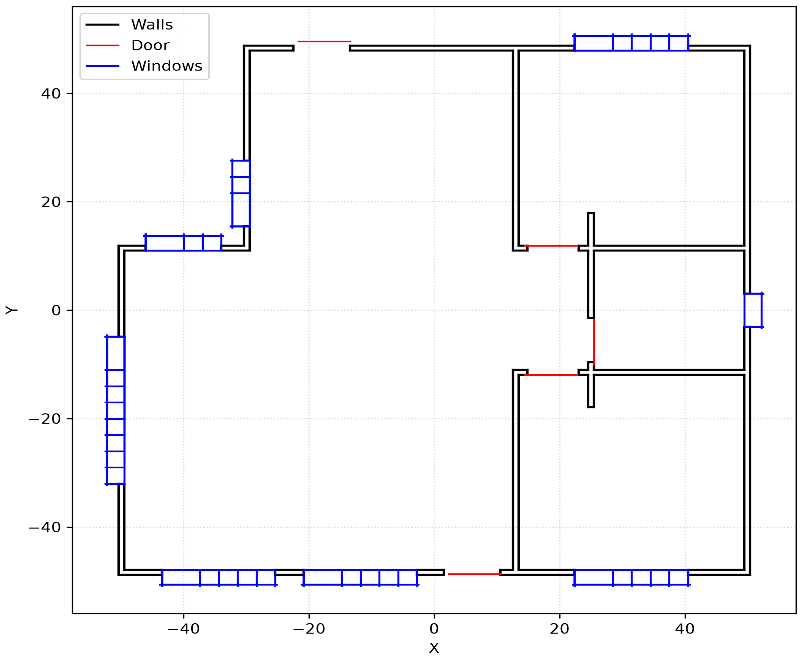
\includegraphics[width=0.7\textwidth]{images/02_geometry_processing/parsing.png}
	\caption{Plot dei segmenti}
	\label{fig:parsing}
\end{figure}
\section{Collasso dei vertici}
\label{sec:snapping}
\section{Ricostruzione delle fessure}
\label{sec:gap_reconstruction}
\section{Estrazione e classificazione delle facce}
\label{sec:face_extraction}
\section{Triangolazione ed estrusione}
\label{sec:triangulation}
\section{Eportazione mesh}
\label{sec:exporting}
    
    \chapter{Generazione della scena e rendering in Blender}
\label{ch:rendering}

\section{Script Python di generazione scena Blender}
\label{sec:script_python_gen_blender_scene}
\section{Setup scena in Blender: materiali, luci, camera, Cycles}
\label{sec:setup_blender}
    
    \chapter{Risultati e valutazione}
\label{ch:results}
    
    \input{chapters/05_conclusioni.tex}

    \input{chapters/99_acknowledgements}
    
    \clearpage 
    
    \addcontentsline{toc}{chapter}{Riferimenti}
    
    \printbibliography[heading=subbibliography, title=Bibliografia]

    \nocite{*}
   
\end{document}